\documentclass{article}

% chinese fonts
\usepackage{ctex}

% math fonts
\usepackage{amsmath}
\usepackage{amsthm}
\usepackage{amssymb}
\usepackage{bm}

% figures
\usepackage{tikz}
\usepackage{graphicx}
\graphicspath{{./figures/}}

% tables
\usepackage{tabularx}
\usepackage{booktabs}

% codes
\usepackage{listings}
\lstset{language     = Matlab,
        basicstyle   = \ttfamily,
        keywordstyle = \color{cyan},
        rulecolor    = \color{black},
        commentstyle = \color{green},
        keepspaces   = true,
        tabsize      = 4,
}

% hyperlinks
\usepackage{hyperref}
\hypersetup{
  breaklinks,
  colorlinks = true,
  citecolor  = blue,
  linkcolor  = red,
  urlcolor   = magenta,
}

% bibliography
\usepackage[sort&compress,numbers]{natbib}

% About:  Macros for Vector, Matrix, Tensor, Math Operator and Misc
% Author: Jingxuan Yang

% vectors
\newcommand{\va}{\bm{a}}       \newcommand{\vah}{\hat{\bm{a}}}        \newcommand{\ah}{\hat{a}}    \newcommand{\vat}{\tilde{\bm{a}}}       \newcommand{\at}{\tilde{a}}
\newcommand{\vb}{\bm{b}}       \newcommand{\vbh}{\hat{\bm{b}}}        \newcommand{\bh}{\hat{b}}    \newcommand{\vbt}{\tilde{\bm{b}}}       \newcommand{\bt}{\tilde{b}}
\newcommand{\vc}{\bm{c}}       \newcommand{\vch}{\hat{\bm{c}}}        \newcommand{\ch}{\hat{c}}    \newcommand{\vct}{\tilde{\bm{c}}}       \newcommand{\ct}{\tilde{c}}
\newcommand{\vd}{\bm{d}}       \newcommand{\vdh}{\hat{\bm{d}}}        \newcommand{\dhat}{\hat{d}}  \newcommand{\vdt}{\tilde{\bm{d}}}       \newcommand{\dt}{\tilde{d}}
\newcommand{\ve}{\bm{e}}       \newcommand{\veh}{\hat{\bm{e}}}        \newcommand{\eh}{\hat{e}}    \newcommand{\vet}{\tilde{\bm{e}}}       \newcommand{\et}{\tilde{e}}
\newcommand{\vf}{\bm{f}}       \newcommand{\vfh}{\hat{\bm{f}}}        \newcommand{\fh}{\hat{f}}    \newcommand{\vft}{\tilde{\bm{f}}}       \newcommand{\ft}{\tilde{f}}
\newcommand{\vg}{\bm{g}}       \newcommand{\vgh}{\hat{\bm{g}}}        \newcommand{\gh}{\hat{g}}    \newcommand{\vgt}{\tilde{\bm{g}}}       \newcommand{\gt}{\tilde{g}}
\newcommand{\vh}{\bm{h}}     \newcommand{\vhh}{\hat{\bm{h}}}        \newcommand{\hh}{\hat{h}}    \newcommand{\vht}{\tilde{\bm{h}}}       \newcommand{\htild}{\tilde{h}}
\newcommand{\vi}{\bm{i}}       \newcommand{\vih}{\hat{\bm{i}}}        \newcommand{\ih}{\hat{i}}    \newcommand{\vit}{\tilde{\bm{i}}}       \newcommand{\itild}{\tilde{i}}
\newcommand{\vj}{\bm{j}}       \newcommand{\vjh}{\hat{\bm{j}}}        \newcommand{\jh}{\hat{j}}    \newcommand{\vjt}{\tilde{\bm{j}}}       \newcommand{\jt}{\tilde{j}}
\newcommand{\vk}{\bm{k}}       \newcommand{\vkh}{\hat{\bm{k}}}        \newcommand{\kh}{\hat{k}}    \newcommand{\vkt}{\tilde{\bm{k}}}       \newcommand{\kt}{\tilde{k}}
\newcommand{\vl}{\bm{l}}       \newcommand{\vlh}{\hat{\bm{l}}}        \newcommand{\lh}{\hat{l}}    \newcommand{\vlt}{\tilde{\bm{l}}}       \newcommand{\lt}{\tilde{l}}
\newcommand{\vm}{\bm{m}}       \newcommand{\vmh}{\hat{\bm{m}}}        \newcommand{\mh}{\hat{m}}    \newcommand{\vmt}{\tilde{\bm{m}}}       \newcommand{\mt}{\tilde{m}}
\newcommand{\vn}{\bm{n}}       \newcommand{\vnh}{\hat{\bm{n}}}        \newcommand{\nh}{\hat{n}}    \newcommand{\vnt}{\tilde{\bm{n}}}       \newcommand{\nt}{\tilde{n}}
\newcommand{\vo}{\bm{o}}       \newcommand{\voh}{\hat{\bm{o}}}        \newcommand{\oh}{\hat{o}}    \newcommand{\vot}{\tilde{\bm{o}}}       \newcommand{\ot}{\tilde{o}}
\newcommand{\vp}{\bm{p}}       \newcommand{\vph}{\hat{\bm{p}}}        \newcommand{\ph}{\hat{p}}    \newcommand{\vpt}{\tilde{\bm{p}}}       \newcommand{\pt}{\tilde{p}}
\newcommand{\vq}{\bm{q}}       \newcommand{\vqh}{\hat{\bm{q}}}        \newcommand{\qh}{\hat{q}}    \newcommand{\vqt}{\tilde{\bm{q}}}       \newcommand{\qt}{\tilde{q}}
\newcommand{\vr}{\bm{r}}       \newcommand{\vrh}{\hat{\bm{r}}}        \newcommand{\rh}{\hat{r}}    \newcommand{\vrt}{\tilde{\bm{r}}}       \newcommand{\rt}{\tilde{r}}
\newcommand{\vs}{\bm{s}}       \newcommand{\vsh}{\hat{\bm{s}}}        \newcommand{\sh}{\hat{s}}    \newcommand{\vst}{\tilde{\bm{s}}}       \newcommand{\st}{\tilde{s}}
\newcommand{\vt}{\bm{t}}       \newcommand{\vth}{\hat{\bm{t}}}        \newcommand{\that}{\hat{t}}  \newcommand{\vtt}{\tilde{\bm{t}}}       \newcommand{\ttil}{\tilde{t}}
\newcommand{\vu}{\bm{u}}       \newcommand{\vuh}{\hat{\bm{u}}}        \newcommand{\uh}{\hat{u}}    \newcommand{\vut}{\tilde{\bm{u}}}       \newcommand{\ut}{\tilde{u}}
\newcommand{\vv}{\bm{v}}       \newcommand{\vvh}{\hat{\bm{v}}}        \newcommand{\vhat}{\hat{v}}    \newcommand{\vvt}{\tilde{\bm{v}}}       \newcommand{\vtild}{\tilde{v}}
\newcommand{\vw}{\bm{w}}       \newcommand{\vwh}{\hat{\bm{w}}}        \newcommand{\wh}{\hat{w}}    \newcommand{\vwt}{\tilde{\bm{w}}}       \newcommand{\wt}{\tilde{w}}
\newcommand{\vx}{\bm{x}}       \newcommand{\vxh}{\hat{\bm{x}}}        \newcommand{\xh}{\hat{x}}    \newcommand{\vxt}{\tilde{\bm{x}}}       \newcommand{\xt}{\tilde{x}}
\newcommand{\vy}{\bm{y}}       \newcommand{\vyh}{\hat{\bm{y}}}        \newcommand{\yh}{\hat{y}}    \newcommand{\vyt}{\tilde{\bm{y}}}       \newcommand{\yt}{\tilde{y}}
\newcommand{\vz}{\bm{z}}       \newcommand{\vzh}{\hat{\bm{z}}}        \newcommand{\zh}{\hat{z}}    \newcommand{\vzt}{\tilde{\bm{z}}}       \newcommand{\zt}{\tilde{z}}

\newcommand{\valpha}{\bm{\alpha}}
\newcommand{\vbeta}{\bm{\beta}}
\newcommand{\vgamma}{\bm{\gamma}}
\newcommand{\vtheta}{\bm{\theta}}
\newcommand{\vlambda}{\bm{\lambda}}
\newcommand{\vmu}{\bm{\mu}}
\newcommand{\vomega}{\bm{\omega}}

\newcommand{\mSigma}{\bm{\Sigma}}

\newcommand{\Fc}{\mathcal{F}}
\newcommand{\Xc}{\mathcal{X}}
\newcommand{\Yc}{\mathcal{Y}}
\newcommand{\Zc}{\mathcal{Z}}
\newcommand{\Gc}{\mathcal{G}}
\newcommand{\Hc}{\mathcal{H}}
\newcommand{\Dc}{\mathcal{D}}
\newcommand{\Cc}{\mathcal{C}}
\newcommand{\Rc}{\mathcal{R}}

% matrices
\newcommand{\ma}{\bm{A}}
\newcommand{\mb}{\bm{B}}
\newcommand{\md}{\bm{D}}
\newcommand{\mH}{\bm{H}}
\newcommand{\mE}{\bm{E}}
\newcommand{\mi}{\bm{I}}
\newcommand{\mk}{\bm{K}}
\newcommand{\ml}{\bm{L}}
\newcommand{\mn}{\bm{N}}
\newcommand{\mP}{\bm{P}}
\newcommand{\mq}{\bm{Q}}
\newcommand{\mr}{\bm{R}}
\newcommand{\mU}{\bm{u}}
\newcommand{\mv}{\bm{v}}
\newcommand{\mw}{\bm{W}}
\newcommand{\mx}{\bm{X}}
\newcommand{\my}{\bm{Y}}
\newcommand{\mz}{\bm{Z}}

% tensors
\newcommand{\tp}{\mathsf{P}}
\newcommand{\tu}{\mathsf{U}}
\newcommand{\tx}{\mathsf{X}}
\newcommand{\ty}{\mathsf{Y}}
\newcommand{\tz}{\mathsf{Z}}
\newcommand{\tw}{\mathsf{W}}
\newcommand{\tf}{\mathsf{F}}
\newcommand{\ta}{\mathsf{A}}
\renewcommand{\th}{\mathsf{H}}

% norms
\newcommand{\mynorm}[2]{\| {#1} \|_{#2}}
\newcommand{\norm}[2]{\mynorm{#1}{#2}}
\newcommand{\bignorm}[2]{\left\| {#1} \right\|_{#2}}
\newcommand{\norml}[1]{\mynorm{#1}{1}}
\newcommand{\bignorml}[1]{\bignorm{#1}{1}}
\newcommand{\infnorm}[1]{\mynorm{#1}{\infty}}
\newcommand{\biginfnorm}[1]{\bignorm{#1}{\infty}}
\newcommand{\oneinf}{\ell_{1,\infty}}
\newcommand{\onetwo}{\ell_{1,2}}
\newcommand{\oneinfnorm}[1]{\mynorm{#1}{1,\infty}}
\newcommand{\bigoneinf}[1]{\bignorm{#1}{1,\infty}}
\newcommand{\onetwonorm}[1]{\mynorm{#1}{1,2}}
\newcommand{\bigonetwo}[1]{\bignorm{#1}{1,2}}
\newcommand{\enorm}[1]{\mynorm{#1}{2}}
\newcommand{\bigenorm}[1]{\bignorm{#1}{2}}
\newcommand{\znorm}[1]{\mynorm{#1}{0}}
\newcommand{\bigznorm}[1]{\bignorm{#1}{0}}
\newcommand{\frob}[1]{\|{#1}\|_{\text{F}}}
\newcommand{\bigfrob}[1]{\bignorm{#1}{\text{F}}}
\newcommand{\grpnorm}[2]{\norm{#1}{\text{Gr}(#2)}}

% math operators
\DeclareMathOperator*{\argmin}{argmin}
\DeclareMathOperator*{\argmax}{argmax}
\DeclareMathOperator{\divg}{div}
\DeclareMathOperator{\dom}{dom}
\DeclareMathOperator{\interior}{int}
\DeclareMathOperator{\ri}{ri}
\DeclareMathOperator{\sgn}{sgn}
\DeclareMathOperator{\trace}{Tr}
\DeclareMathOperator{\diag}{diag}
\DeclareMathOperator{\rank}{rank}
\DeclareMathOperator{\range}{range}
\DeclareMathOperator{\vect}{vec}
\DeclareMathOperator{\prox}{prox}
\DeclareMathOperator{\intr}{int}
\DeclareMathOperator{\relint}{ri}

% misc
\newcommand{\gs}{\geqslant}
\newcommand{\ls}{\leqslant}
\newcommand{\set}[1]{\left\{ {#1}\right\}}

\newcommand{\defeq}{\ \stackrel{\text{def}}{=}\ }
\newcommand{\ip}[2]{\left\langle#1, #2\right\rangle}
\newcommand{\reals}{\mathbb{R}}
\newcommand{\complex}{\mathbb{C}}
\newcommand{\half}{\frac{1}{2}}

\newtheorem{theorem}{Theorem}
\newtheorem{lemma}[theorem]{Lemma}
\newtheorem{proposition}[theorem]{Proposition}
\newtheorem{remark}[theorem]{Remark}
\newtheorem{corollary}[theorem]{Corollary}
\newtheorem{definition}[theorem]{Definition}


\setlength{\oddsidemargin}{-0.25 in}
\setlength{\evensidemargin}{-0.25 in} 
\setlength{\topmargin}{-0.25in} 
\setlength{\textwidth}{7 in} 
\setlength{\textheight}{8.5 in}
\setlength{\headsep}{0.25 in} 
\setlength{\parindent}{0 in}
\setlength{\parskip}{0.1 in}

\newcommand{\homework}[5]{
  \pagestyle{myheadings} 
  \thispagestyle{plain}
  \newpage
  \setcounter{page}{1} 
  \setcounter{section}{#5} 
  \noindent
  \begin{center}
    \framebox{ 
      \vbox{
        \vspace{2mm} 
        \hbox to 6.28in { {\bf
        THU-70250043-0,~Pattern~Recognition~(Spring 2021) \hfill Homework: 3} }
        \vspace{6mm} 
        \hbox to 6.28in { {\Large \hfill #1 \hfill} }
        \vspace{6mm} 
        \hbox to 6.28in { {\it Lecturer: #2 \hfill} }
        \vspace{2mm} 
        \hbox to 6.28in { {\it \hspace{14mm} #3 \hfill} }
        \vspace{2mm} 
        \hbox to 6.28in { {\it Student: #4 \hfill} }
        \vspace{2mm} 
      } 
    }
  \end{center}
  \markboth{#1}{#1} 
  \vspace*{4mm} 
}

\begin{document}

\homework{GMM and EM}{Changshui Zhang
\hspace{5mm} {\tt zcs@mail.tsinghua.edu.cn}}{Hong Zhao \hspace{16mm} {\tt vzhao@tsinghua.edu.cn}}{Jingxuan Yang \hspace{10mm} {\tt yangjx20@mails.tsinghua.edu.cn}}{8}

\section*{EM and GD}

1. In this problem you will see connections between the EM algorithm and gradient descent. Consider a GMM with known mixture weight $\pi_k$ and spherical covariances (but the radius of spheres might be different). Its log likelihood is given by
\begin{equation}
	l\left(\left\{\mu_k,\sigma_k^2\right\}_{k=1}^K\right) = \sum_{i=1}^n\log\left(\sum_{k=1}^K\pi_k N(x_i|\mu_k,\sigma_k^2I)\right).
\end{equation}

A maximization algorithm based on gradient descent should be something like:
\begin{itemize}
	\item Initialize $\mu_k$ and $\sigma_k^2$, $k \in\{1,2,\cdots,K\}$. Set the iteration counter $t\leftarrow1$.
	\item Repeat the following until convergence:
	\begin{itemize}
		\item For $k=1,2,\cdots ,K$,
      \begin{equation}
        \mu_k^{(t+1)}\leftarrow\mu_k^{(t)}+\eta_k^{(t)}\nabla_{\mu_k}l\left(\left\{\mu_k^{(t)},(\sigma_k ^2)^{(t)}\right\}_{k=1}^K\right)
      \end{equation}
		\item For $k=1,2,\cdots ,K$,
      \begin{equation}
        (\sigma_k ^2)^{(t+1)} \leftarrow (\sigma_k ^2)^{(t)}+s_k^{(t)}\nabla_{\sigma_k^2}l\left(\left\{\mu_k^{(t+1)},(\sigma_k ^2)^{(t)}\right\}_{k=1}^K\right)
      \end{equation}
		\item Increase the iteration counter $t\leftarrow t+1$.
	\end{itemize}
\end{itemize}

Please prove that with properly chosen step size $\eta_k^{(t)}$ and $s_k^{(t)}$, the above gradient descent algorithm is essentially equivalent to the following \emph{modified} EM algorithm:
\begin{itemize}
	\item Initialize $\mu_k$ and $\sigma_k^2$, $k \in \{1,2,\cdots ,K\}$. Set the iteration counter $t\leftarrow1$.
	\item Repeat the following until convergence:
	\begin{itemize}
		\item E-step:
      \begin{equation}
        \tilde{z}_{ik}^{(t+0.5)} \leftarrow P\left(x_i\in \mathrm{cluster}_k \Big| \left\{\mu_j^{(t)},(\sigma_j^2)^{(t)}\right\}_{j=1}^K,x_i\right)
      \end{equation}
		\item M-step:
      \begin{equation}
        \left\{\mu_k^{(t+1)}\right\}_{k=1}^K \leftarrow \argmax_{\{\mu_k\}_{k=1}^K} \sum_{i=1}^n\sum_{k=1}^K \tilde{z}_{ik}^{(t+0.5)} \left[\log N\left(x_i\Big|\mu_k,(\sigma_k^2)^{(t)}I\right)+\log\pi_k\right]
      \end{equation}
		\item E-step:
      \begin{equation}
        \tilde{z}_{ik}^{(t+1)} \leftarrow P\left(x_i \in \mathrm{cluster}_k \Big| \left\{\mu_j^{(t+1)},(\sigma_j^2)^{(t)}\right\}_{j=1}^K,x_i\right)
      \end{equation}
		\item M-step:
      \begin{equation}
        \left\{(\sigma_k^2)^{(t+1)}\right\}_{k=1}^K \leftarrow \argmax_{\{\sigma_k^2\}_{k=1}^K} \sum_{i=1}^n \sum_{k=1}^K \tilde{z}_{ik}^{(t+1)} \left[\log N\left(x_i\Big|\mu_k^{(t+1)},\sigma_k^2I\right)+\log \pi_k \right]
      \end{equation}
		\item Increase the iteration counter $t\leftarrow t+1$.
	\end{itemize}
\end{itemize}

The main modification is inserting an extra E-step between the M-step for $\mu_k$'s and the M-step for $\sigma_k^2$'s.

\emph{Hint:} Find the exact algebraic form of step size $\eta_k^{(t)}$ and $s_k^{(t)}$ from M-step.

解: 设样本点 $x_i$ 的维数为 $d$, 则正态分布概率密度为
\begin{equation}
  N(x_i|\mu_k,\sigma_k^2I)=\frac{1}{(2\pi\sigma_k^2)^{d/2}}\exp\left[-\frac{1}{2\sigma_k^2}(x_i-\mu_k)^{\top}(x_i-\mu_k)\right]
\end{equation}

其对 $\mu_k$ 的梯度为
\begin{equation}
  \nabla_{\mu_k}N(x_i|\mu_k,\sigma_k^2I)
  =N(x_i|\mu_k,\sigma_k^2I)\frac{x_i-\mu_k}{\sigma_k^2}
\end{equation}

对 $\sigma_k^2$ 的梯度为
\begin{equation}
  \begin{aligned}
    \nabla_{\sigma_k^2}N(x_i|\mu_k,\sigma_k^2I)
    &=N(x_i|\mu_k,\sigma_k^2I)\left[-\frac{d}{2\sigma_k^2}+\frac{1}{2(\sigma_k^2)^2}(x_i-\mu_k)^{\top}(x_i-\mu_k)\right]
  \end{aligned}
\end{equation}

所以, 似然函数对 $\mu_k$ 的梯度为
\begin{equation}
  \begin{aligned}
    \nabla_{\mu_k}l\left(\left\{\mu_k,\sigma_k ^2\right\}_{k=1}^K\right)
    &=\nabla_{\mu_k} \sum_{i=1}^n \log\left(\sum_{k=1}^K\pi_k N(x_i|\mu_k,\sigma_k^2I)\right)\\
    &=\sum_{i=1}^n\frac{\pi_k N(x_i|\mu_k,\sigma_k^2I)}{\displaystyle\sum_{k=1}^K\pi_k N(x_i|\mu_k,\sigma_k^2I)}\frac{x_i-\mu_k}{\sigma_k^2}\\
  \end{aligned}
\end{equation}

似然函数对 $\sigma_k^2$ 的梯度为
\begin{equation}
  \begin{aligned}
    \nabla_{\sigma_k^2}l\left(\left\{\mu_k,\sigma_k^2\right\}_{k=1}^K\right)
    &=\nabla_{\sigma_k^2} \sum_{i=1}^n \log\left(\sum_{k=1}^K\pi_k N(x_i|\mu_k,\sigma_k^2I)\right)\\
    &=\sum_{i=1}^n \frac{\pi_k N(x_i|\mu_k,\sigma_k^2I)}{\displaystyle\sum_{k=1}^K\pi_k N(x_i|\mu_k,\sigma_k^2I)}\left[-\frac{d}{2\sigma_k^2}+\frac{1}{2(\sigma_k^2)^2}(x_i-\mu_k)^{\top}(x_i-\mu_k)\right]\\
  \end{aligned}
\end{equation}

对改进 EM 算法, 第一个 E-step: 由 Bayes 公式可得
\begin{equation}
  \begin{aligned}
    \tilde{z}_{ik}^{(t+0.5)} 
    &=P\left(x_i\in \mathrm{cluster}_k \Big| \left\{\mu_j^{(t)},(\sigma_j^2)^{(t)}\right\}_{j=1}^K,x_i\right)\\
    &=\frac{\pi_k N\left(x_i\Big|\mu_k^{(t)},(\sigma_k^2)^{(t)}I\right)}{\displaystyle\sum_{k=1}^K\pi_k N\left(x_i\Big|\mu_k^{(t)},(\sigma_k^2)^{(t)}I\right)}
  \end{aligned}
\end{equation}

第一个 M-step: 令
\begin{equation}
    Q^{(t+0.5)}\triangleq\sum_{i=1}^n\sum_{k=1}^K \tilde{z}_{ik}^{(t+0.5)} \left[\log N\left(x_i\Big|\mu_k,(\sigma_k^2)^{(t)}I\right)+\log\pi_k\right]
\end{equation}

则其对 $\mu_k$ 的梯度为
\begin{equation}
  \begin{aligned}
    \frac{\partial Q^{(t+0.5)}}{\partial \mu_k}
    &=\sum_{i=1}^n\tilde{z}_{ik}^{(t+0.5)}\frac{N\left(x_i\Big|\mu_k,(\sigma_k^2)^{(t)}I\right)}{N\left(x_i\Big|\mu_k,(\sigma_k^2)^{(t)}I\right)}\frac{x_i-\mu_k}{(\sigma_k^2)^{(t)}}\\
    &=\sum_{i=1}^n\tilde{z}_{ik}^{(t+0.5)}\frac{x_i-\mu_k}{(\sigma_k^2)^{(t)}}\\
    &=\frac{1}{(\sigma_k^2)^{(t)}}\left(\sum_{i=1}^n\tilde{z}_{ik}^{(t+0.5)}x_i-\sum_{i=1}^n\tilde{z}_{ik}^{(t+0.5)}\mu_k\right)
  \end{aligned}
\end{equation}

令此梯度为 0, 则有
\begin{equation}
  \mu_k^{(t+1)}=\frac{\displaystyle\sum_{i=1}^n\tilde{z}_{ik}^{(t+0.5)}x_i}{\displaystyle\sum_{i=1}^n\tilde{z}_{ik}^{(t+0.5)}}
\end{equation}

对梯度下降算法, $\mu_k^{(t+1)}$ 为
\begin{equation}
  \begin{aligned}
    \mu_k^{(t+1)}
    &=\mu_k^{(t)}+\eta_k^{(t)}\nabla_{\mu_k}l\left(\left\{\mu_k^{(t)},(\sigma_k ^2)^{(t)}\right\}_{k=1}^K\right)\\
    &=\mu_k^{(t)}+\eta_k^{(t)}\sum_{i=1}^n\frac{\pi_k N\left(x_i\Big|\mu_k^{(t)},(\sigma_k^2)^{(t)}I\right)}{\displaystyle\sum_{k=1}^K\pi_k N\left(x_i\Big|\mu_k^{(t)},(\sigma_k^2)^{(t)}I\right)}\frac{x_i-\mu_k^{(t)}}{(\sigma_k ^2)^{(t)}}\\
    &=\mu_k^{(t)}+\eta_k^{(t)}\sum_{i=1}^n\tilde{z}_{ik}^{(t+0.5)}\frac{x_i-\mu_k^{(t)}}{(\sigma_k ^2)^{(t)}}\\
  \end{aligned}
\end{equation}

令梯度下降算法得到的 $\mu_k^{(t+1)}$ 与 EM 算法得到的结果相等, 则有
\begin{equation}
  \frac{\displaystyle\sum_{i=1}^n\tilde{z}_{ik}^{(t+0.5)}x_i}{\displaystyle\sum_{j=1}^n\tilde{z}_{jk}^{(t+0.5)}}
  =\mu_k^{(t)}+\eta_k^{(t)}\sum_{i=1}^n\tilde{z}_{ik}^{(t+0.5)}\frac{x_i-\mu_k^{(t)}}{(\sigma_k ^2)^{(t)}}
\end{equation}

通分有
\begin{equation}
  \sum_{i=1}^n\tilde{z}_{ik}^{(t+0.5)}x_i
  =\sum_{j=1}^n\tilde{z}_{jk}^{(t+0.5)}\mu_k^{(t)}+\sum_{j=1}^n\tilde{z}_{jk}^{(t+0.5)}\eta_k^{(t)}\sum_{i=1}^n\tilde{z}_{ik}^{(t+0.5)}\frac{x_i-\mu_k^{(t)}}{(\sigma_k ^2)^{(t)}}
\end{equation}

移项可得
\begin{equation}
  \sum_{i=1}^n\tilde{z}_{ik}^{(t+0.5)}\left(x_i-\mu_k^{(t)}\right)
  =\frac{\eta_k^{(t)}\displaystyle\sum_{j=1}^n\tilde{z}_{jk}^{(t+0.5)}}{(\sigma_k ^2)^{(t)}}\sum_{i=1}^n\tilde{z}_{ik}^{(t+0.5)}\left(x_i-\mu_k^{(t)}\right)
\end{equation}

即
\begin{equation}
  \frac{\eta_k^{(t)}\displaystyle\sum_{j=1}^n\tilde{z}_{jk}^{(t+0.5)}}{(\sigma_k ^2)^{(t)}}=1
\end{equation}

所以
\begin{equation}
  \eta_k^{(t)}=\frac{(\sigma_k ^2)^{(t)}}{\displaystyle\sum_{j=1}^n\tilde{z}_{jk}^{(t+0.5)}}
\end{equation}

对改进 EM 算法, 第二个 E-step: 由 Bayes 公式可得
\begin{equation}
  \begin{aligned}
    \tilde{z}_{ik}^{(t+1)} 
    &=P\left(x_i\in \mathrm{cluster}_k \Big| \left\{\mu_j^{(t+1)},(\sigma_j^2)^{(t)}\right\}_{j=1}^K,x_i\right)\\
    &=\frac{\pi_k N\left(x_i\Big|\mu_k^{(t+1)},(\sigma_k^2)^{(t)}I\right)}{\displaystyle\sum_{k=1}^K\pi_k N\left(x_i\Big|\mu_k^{(t+1)},(\sigma_k^2)^{(t)}I\right)}
  \end{aligned}
\end{equation}

第二个 M-step: 令
\begin{equation}
    Q^{(t+1)}\triangleq\sum_{i=1}^n\sum_{k=1}^K \tilde{z}_{ik}^{(t+1)} \left[\log N\left(x_i\Big|\mu_k^{(t+1)},\sigma_k^2I\right)+\log\pi_k\right]
\end{equation}

则其对 $\sigma_k^2$ 的梯度为
\begin{equation}
  \begin{aligned}
    \frac{\partial Q^{(t+1)}}{\partial \sigma_k^2}
    &=\sum_{i=1}^n\tilde{z}_{ik}^{(t+1)}\frac{N\left(x_i\Big|\mu_k^{(t+1)},\sigma_k^2I\right)}{N\left(x_i\Big|\mu_k^{(t+1)},\sigma_k^2I\right)}\left[-\frac{d}{2\sigma_k^2}+\frac{1}{2(\sigma_k^2)^2}\left(x_i-\mu_k^{(t+1)}\right)^{\top}\left(x_i-\mu_k^{(t+1)}\right)\right]\\
    &=\sum_{i=1}^n\tilde{z}_{ik}^{(t+1)}\left[-\frac{d}{2\sigma_k^2}+\frac{1}{2(\sigma_k^2)^2}\left(x_i-\mu_k^{(t+1)}\right)^{\top}\left(x_i-\mu_k^{(t+1)}\right)\right]\\
    &=\frac{1}{2(\sigma_k^2)^2}\left[\sum_{i=1}^n\tilde{z}_{ik}^{(t+1)}\left\|x_i-\mu_k^{(t+1)}\right\|^2-\sigma_k^2d\sum_{i=1}^n\tilde{z}_{ik}^{(t+1)}\right]
  \end{aligned}
\end{equation}

令此梯度为 0, 则有
\begin{equation}
  (\sigma_k^2)^{(t+1)}=\frac{\displaystyle\sum_{i=1}^n\tilde{z}_{ik}^{(t+1)}\left\|x_i-\mu_k^{(t+1)}\right\|^2}{\displaystyle d\sum_{i=1}^n\tilde{z}_{ik}^{(t+1)}}
\end{equation}

对梯度下降算法, $(\sigma_k^2)^{(t+1)}$ 为
\begin{equation}
  \begin{aligned}
    (\sigma_k^2)^{(t+1)}
    &=(\sigma_k ^2)^{(t)}+s_k^{(t)}\nabla_{\sigma_k^2}l\left(\left\{\mu_k^{(t+1)},(\sigma_k^2)^{(t)}\right\}_{k=1}^K\right)\\
    &=(\sigma_k^2)^{(t)}+s_k^{(t)}\sum_{i=1}^n \frac{\pi_k N\left(x_i\Big|\mu_k^{(t+1)},(\sigma_k^2)^{(t)}I\right)}{\displaystyle\sum_{k=1}^K\pi_k N\left(x_i\Big|\mu_k^{(t+1)},(\sigma_k^2)^{(t)}I\right)}\left[-\frac{d}{2(\sigma_k^2)^{(t)}}+\frac{\left\|x_i-\mu_k^{(t+1)}\right\|^2}{2\big[(\sigma_k^2)^{(t)}\big]^2}\right]\\
    &=(\sigma_k ^2)^{(t)}+s_k^{(t)}\sum_{i=1}^n \tilde{z}_{ik}^{(t+1)}\left[-\frac{d}{2(\sigma_k^2)^{(t)}}+\frac{1}{2\big[(\sigma_k^2)^{(t)}\big]^2}\left\|x_i-\mu_k^{(t+1)}\right\|^2\right]\\
  \end{aligned}
\end{equation}

令梯度下降算法得到的 $(\sigma_k^2)^{(t+1)}$ 与 EM 算法得到的结果相等, 则有
\begin{equation}
  \frac{\displaystyle\sum_{i=1}^n\tilde{z}_{ik}^{(t+1)}\left\|x_i-\mu_k^{(t+1)}\right\|^2}{\displaystyle d\sum_{j=1}^n\tilde{z}_{jk}^{(t+1)}}
  =(\sigma_k ^2)^{(t)}+s_k^{(t)}\sum_{i=1}^n \tilde{z}_{ik}^{(t+1)}\left[-\frac{d}{2(\sigma_k^2)^{(t)}}+\frac{1}{2\big[(\sigma_k^2)^{(t)}\big]^2}\left\|x_i-\mu_k^{(t+1)}\right\|^2\right]
\end{equation}

通分并移项可得
\begin{equation}
  \sum_{i=1}^n\tilde{z}_{ik}^{(t+1)}\left(\left\|x_i-\mu_k^{(t+1)}\right\|^2-d(\sigma_k ^2)^{(t)}\right)
  =\frac{\displaystyle s_k^{(t)}d\sum_{j=1}^n\tilde{z}_{jk}^{(t+1)}}{2\big[(\sigma_k^2)^{(t)}\big]^2}\sum_{i=1}^n\tilde{z}_{ik}^{(t+1)}\left(\left\|x_i-\mu_k^{(t+1)}\right\|^2-d(\sigma_k ^2)^{(t)}\right)
\end{equation}

即
\begin{equation}
  \frac{\displaystyle s_k^{(t)}d\sum_{j=1}^n\tilde{z}_{jk}^{(t+1)}}{2\big[(\sigma_k^2)^{(t)}\big]^2}=1
\end{equation}

所以
\begin{equation}
  s_k^{(t)}=\frac{2\big[(\sigma_k^2)^{(t)}\big]^2}{\displaystyle d\sum_{j=1}^n\tilde{z}_{jk}^{(t+1)}}
\end{equation}

综上所述, 若取步长分别为
\begin{equation}
  \eta_k^{(t)}=\frac{(\sigma_k ^2)^{(t)}}{\displaystyle\sum_{j=1}^n\tilde{z}_{jk}^{(t+0.5)}},\quad s_k^{(t)}=\frac{2\big[(\sigma_k^2)^{(t)}\big]^2}{\displaystyle d\sum_{j=1}^n\tilde{z}_{jk}^{(t+1)}}
\end{equation}

则梯度下降算法与改进 EM 算法本质上是等价的.

\section*{EM for MAP Estimation}

2. The EM algorithm that we talked about in class was for solving a maximum likelihood estimation problem in which we wished to maximize
\begin{equation}
  \prod_{i = 1}^mp(x^{(i)}|\theta) = \prod_{i = 1}^m \sum_{z^{(i)}}p(x^{(i)},z^{(i)}|\theta)
\end{equation}
where $x^{(i)}$ were visible variables, $z^{(i)}$ were hidden variables and $m$ was the number of samples. Suppose we are working in a Bayesian framework, and wanted to find the MAP estimate of the parameters $\theta$ by maximizing
\begin{equation}
  \left(\prod_{i = 1}^mp(x^{(i)}|\theta)\right)p(\theta) = \left(\prod_{i = 1}^m \sum_{z^{(i)}}p(x^{(i)},z^{(i)}|\theta)\right)p(\theta)
  \label{eq:llhmap}
\end{equation}

Here, $p(\theta)$ is our prior on the parameters. Please generalize the EM algorithm to work for MAP estimation. You may assume that $\log p(x,z|\theta)$ and $\log p(\theta)$ are both concave in $\theta$, so that the M-step is tractable if it requires only maximizing a linear combination of these quantities. (This roughly corresponds to assuming that MAP estimation is tractable when $x, z$ is fully observed, just like in the frequentist case where we considered examples in which maximum likelihood estimation was easy if $x, z$ was fully observed.)

Make sure your M-step is tractable, and also prove that $\displaystyle\left(\prod_{i = 1}^mp(x^{(i)}|\theta)\right)p(\theta)$ (viewed as a function of $\theta$) monotonically increases with each iteration of your algorithm.

解: 令 $X=\left\{x^{(1)},x^{(2)},\cdots,x^{(m)}\right\}$, 对式 (\ref{eq:llhmap}) 取自然对数可得
\begin{equation}
  \begin{aligned}
    \tilde{H}(\theta)
    &=\log\big[p(X|\theta)p(\theta)\big]\\
    &=\log\left[\left(\prod_{i = 1}^mp(x^{(i)}|\theta)\right)p(\theta)\right]\\
    &=\log\left[\left(\prod_{i = 1}^m \sum_{z^{(i)}}p(x^{(i)},z^{(i)}|\theta)\right)p(\theta)\right]\\
    &=\sum_{i=1}^m\log\sum_{z^{(i)}}p\left(x^{(i)},z^{(i)}|\theta\right)+\log p(\theta)\\
  \end{aligned}
\end{equation}

引入隐变量分布 $q(\cdot)$, 由 Jensen 不等式可得
\begin{equation}
  \tilde{H}(\theta)
  \gs\sum_{i=1}^m\sum_{z^{(i)}}q(z^{(i)})\log p\left(x^{(i)},z^{(i)}|\theta\right)-\sum_{i=1}^m\sum_{z^{(i)}}q(z^{(i)})\log q(z^{(i)})+\log p(\theta)
  \triangleq \tilde{F}(q,\theta)
\end{equation}

直接优化 $\tilde{H}(\theta)$ 可能是很困难的, 所以我们转而优化 $\tilde{H}(\theta)$ 的下界函数 $\tilde{F}(q,\theta)$. 优化函数 $\tilde{F}(q,\theta)$ 可能也是比较困难的, 因此我们采用一种简单的迭代算法对 $\tilde{F}(q,\theta)$ 寻优, 首先对变量 $q,~\theta$ 初始化, 然后固定变量 $\theta_{[k]}$ 寻找能够最大化函数 $\tilde{F}(q,\theta_{[k]})$ 的参数 $q_{[k+1]}$, 再固定参数 $q_{[k+1]}$ 寻找能够最大化函数 $\tilde{F}(q_{[k+1]},\theta)$ 的参数 $\theta_{[k+1]}$, 即反复执行下面的两个步骤:
\begin{equation}
  q_{[k+1]}\leftarrow\argmax_{q}\tilde{F}(q,\theta_{[k]})
  \label{eq:estep}
\end{equation}
\begin{equation}
  \theta_{[k+1]}\leftarrow\argmax_{\theta}\tilde{F}(q_{[k+1]},\theta)
\end{equation}

当 $q_{[k+1]}(z^{(i)})=p(z^{(i)}|x^{(i)},\theta_{[k]})$ 时, 式 (\ref{eq:estep}) 取到最大值, 因为此时有
\begin{equation}
  \begin{aligned}
    \tilde{F}(q_{[k+1]},\theta_{[k]})
    &=\sum_{i=1}^m\sum_{z^{(i)}}q_{[k+1]}(z^{(i)})\log \frac{p\left(x^{(i)},z^{(i)}|\theta_{[k]}\right)}{q_{[k+1]}(z^{(i)})}+\log p(\theta_{[k]})\\
    &=\sum_{i=1}^m\sum_{z^{(i)}}p(z^{(i)}|x^{(i)},\theta_{[k]})\log \frac{p(z^{(i)}|x^{(i)},\theta_{[k]})p(x^{(i)}|\theta_{[k]})}{p(z^{(i)}|x^{(i)},\theta_{[k]})}+\log p(\theta_{[k]})\\
    &=\sum_{i=1}^m\sum_{z^{(i)}}p(z^{(i)}|x^{(i)},\theta_{[k]})\log p(x^{(i)}|\theta_{[k]})+\log p(\theta_{[k]})\\
    &=\sum_{i=1}^m\log p(x^{(i)}|\theta_{[k]})+\log p(\theta_{[k]})\\
    &=\log\left[\left(\prod_{i = 1}^mp(x^{(i)}|\theta_{[k]})\right)p(\theta_{[k]})\right]\\
    &=\tilde{H}(\theta_{[k]})
  \end{aligned}
  \label{eq:posterior}
\end{equation}

当 $q_{[k+1]}(z^{(i)})=p(z^{(i)}|x^{(i)},\theta_{[k]})$ 时, 
\begin{equation}
  \tilde{F}(q_{[k+1]},\theta)=\sum_{i=1}^m\sum_{z^{(i)}}q_{[k+1]}(z^{(i)})\log p\left(x^{(i)},z^{(i)}|\theta\right)-\sum_{i=1}^m\sum_{z^{(i)}}q_{[k+1]}(z^{(i)})\log q_{[k+1]}(z^{(i)})+\log p(\theta)
\end{equation}

由于第二项不包含需要优化的变量 $\theta$, 则可定义
\begin{equation}
  \tilde{Q}(\theta_{[k]},\theta)=\sum_{i=1}^m\sum_{z^{(i)}}p(z^{(i)}|x^{(i)},\theta_{[k]})\log p\left(x^{(i)},z^{(i)}|\theta\right)+\log p(\theta)
\end{equation}

假设 $\log p(x,z|\theta)$ 和 $\log p(\theta)$ 都是 $\theta$ 的凹函数, 则最大化函数 $\tilde{Q}$ 是一个无约束的凸优化问题, 即 M-step 是容易处理的 (tractable).

综上, 广义 EM 算法为:
\begin{itemize}
  \item 初始化变量 $q,~\theta$
  \item E 步骤, 计算函数 
    \begin{equation}
      \tilde{Q}(\theta_{[k]},\theta)=\sum_{i=1}^m\sum_{z^{(i)}}p(z^{(i)}|x^{(i)},\theta_{[k]})\log p\left(x^{(i)},z^{(i)}|\theta\right)+\log p(\theta)
    \end{equation}
  \item M 步骤, 
    \begin{equation}
      \theta_{[k+1]}\leftarrow\argmax_{\theta}\tilde{Q}(\theta_{[k]},\theta)
    \end{equation}
  \item 如果算法收敛则停止, 否则回到 E 步骤.
\end{itemize}

下面证明在广义 EM 算法下, $\displaystyle\left(\prod_{i = 1}^mp(x^{(i)}|\theta)\right)p(\theta)$ 作为 $\theta$ 的函数的单调性. 由式 (\ref{eq:posterior}) 并结合广义 EM 算法不断迭代求最大值可知
\begin{equation}
  \tilde{H}(\theta_{[k]})=\tilde{F}(q_{[k+1]},\theta_{[k]})\ls\tilde{F}(q_{[k+1]},\theta_{[k+1]})\ls\tilde{F}(q_{[k+2]},\theta_{[k+1]})=\tilde{H}(\theta_{[k+1]}),\quad\forall~k\gs1
\end{equation}

所以, 函数
\begin{equation*}
  \tilde{H}(\theta)=\log\left[\left(\prod_{i = 1}^mp(x^{(i)}|\theta)\right)p(\theta)\right]
\end{equation*}
随着算法的迭代是单调递增的, 又 自然对数函数是一一映射, 则 $\displaystyle\left(\prod_{i = 1}^mp(x^{(i)}|\theta)\right)p(\theta)$ 作为 $\theta$ 的函数也是随着算法的迭代单调递增的.

\section*{Programming 1 (EM and GMM)}

3. Consider the case that the hidden variable $y \in \{1,2,\cdots,m\}$ is discrete while the visible variable $x \in R^d$ is continuous. In other words, we consider mixture models of the form
\begin{equation}
	p(x) = \sum_{j = 1}^m p(x|y = j)p(y=j)
\end{equation}

We assume throughout that $x$ is conditionally Gaussian in the sense that $x \sim \mathcal{N}(\mu_j, \Sigma_j)$ when $y = j$. We have provided you with an example EM code for mixture of Gaussians (with visualization) in MATLAB. The command to run is: 

\verb|[param,history,ll] = em_mix(data,m,eps);| 

where the input points are given as rows of \verb|data|, \verb|m| is the number of components in the estimated mixture, and \verb|eps| determines the stopping criteria of EM: the algorithm stops when the relative change in log-likelihood falls below \verb|eps|. In the output, \verb|param| is a cell array with \verb|m| elements. Each element is a structure with the following fields:

\verb|mean| - the resulting mean of the Gaussian component,

\verb|cov| - the resulting covariance matrix of the component,

\verb|p| - the resulting estimate of the mixing parameter.

The value of \verb|param| is updated after every iteration of EM; the output argument \verb|history| contains copies of these subsequent values of \verb|param| and allows to analyze our experiments. Finally, \verb|ll| is the vector where the $t^{\mathrm{th}}$ element is the value of the log-likelihood of the \verb|data| after $t$ iterations (i.e. the last element is the final log-likelihood of the fitted mixture of Gaussians).

\emph{Hint:} For the following two questions you are encouraged to google ``BIC (Bayesian Information Criterion)'' to help you with the model selection process. Of course other criteria are welcomed as long as you give convincing reasons.

\emph{Hint:} For this assignment, you are allowed to implement EM algorithm manually in python, and you can use scipy.io.loadmat to load the data.

3.1. Run the EM algorithm based on \verb|data| provided by \verb|emdata.mat| with \verb|m = 2, 3, 4, 5| components. Select the appropriate model (number of components) and give reasons for your choice. Note that you may have to rerun the algorithm a few times (and select the model with the highest log-likelihood) for each choice of \verb|m| as EM can sometimes get stuck in a local minimum. Is the model selection result sensible based on what you would expect visually? Why or why not?

解: 对每个 $m$ 进行 10 次测试, 选择对数似然概率最大的那次测试结果作为该组的结果, 如图 \ref{fig:gmmem1} 所示. 

\begin{figure}[htbp]
  \centering
  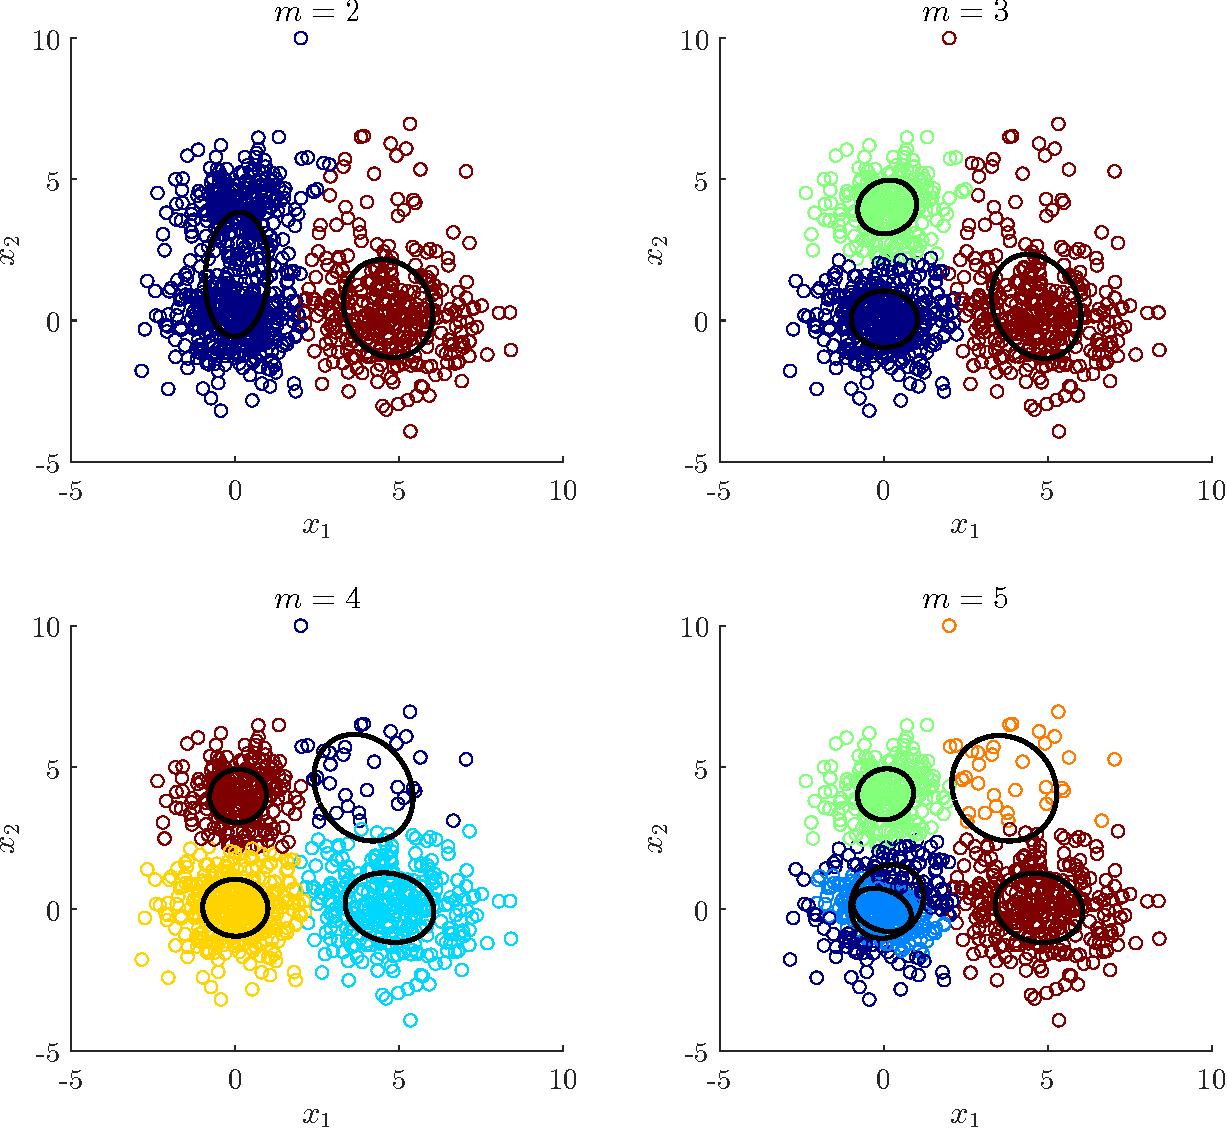
\includegraphics[width=6in]{gmmem-1.pdf}
  \caption{使用 EM 算法对 GMM 模型进行估计}
  \label{fig:gmmem1}
\end{figure}

选择 BIC 作为模型参数选择依据, 
\begin{equation}
  \mathrm{BIC}=k\ln n-2\ln\hat{l}
\end{equation}
其中, $n$ 为数据点个数, $\hat{l}$ 为对数似然概率, $k$ 为模型估计的变量个数, 其中分配概率为 1, 均值为 2, 协方差对称矩阵为 $4-1=3$, 又因为分配概率之和固定 ($=1$) 则最后需 $-1$,
\begin{equation}
  k=(1+d+d^2-1)m-1=6m-1
\end{equation}
其中, $d$ 为数据点维数, 此处为 $d=2$.

BIC 计算结果如表 \ref{tab:bic} 所示, 可知当 $m=4$ 时, BIC 最小, 即 $m=4$ 是最恰当的模型参数. 

\begin{table}[htbp]
  \centering
  \caption{不同参数 $m$ 取值对应的 BIC 数值}
  \label{tab:bic}
  \begin{tabular}{ccccc}
    \hline
        & $m=2$ & $m=3$ & $m=4$ & $m=5$ \\
    \hline
    BIC & 8542.29 & 8371.61 & 8330.65 & 8372.01\\
    \hline
  \end{tabular}
\end{table}

此模型选择结果与视觉预估不符, 在初看数据时, 可以发现有 3 个明显的数据聚集中心, 因此猜测 $m=3$ 是最恰当的模型参数. 但是程序运行结果表明 $m=4$ 是最恰当的模型参数, 这是因为右上角那部分点虽然不够集中, 但是比较不容易被另外三个组分共同作用而产生, 相反若右上角存在一个单独的组分, 并且赋予其很小的比例系数, 则会使得模型拟合效果更好.

3.2. Modify the M-step of the EM code so that the covariance matrices of the Gaussian components are constrained to be equal. Give detailed derivation. Rerun the code and then select an appropriate model. Would we select a different number of components in this case?

解: EM 算法的 M-step 为
\begin{equation}
  \Theta^{(i)}=\argmax_{\Theta} Q(\Theta,\Theta^{(i-1)})
\end{equation}

设 GMM 模型为
\begin{equation}
  p(\vx|\Theta)=\sum_{i=1}^M\alpha_ip_i(\vx|\theta_i)
\end{equation}

则有
\begin{equation}
  \begin{aligned}
    Q(\Theta,\Theta^g)
    &=\sum_{l=1}^M\sum_{i=1}^N\log(\alpha_lp_l(x_i|\theta_l))p(l|x_i,\Theta^g)\\
    &=\sum_{l=1}^M\sum_{i=1}^N\log(\alpha_l)p(l|x_i,\Theta^g)+\sum_{l=1}^M\sum_{i=1}^N\log(p_l(x_i|\theta_l))p(l|x_i,\Theta^g)
  \end{aligned}
\end{equation}

其中第一项不含 $\theta_l$, 第二项不含 $\alpha_l$, 则可在优化 $Q(\Theta,\Theta^g)$ 时分别进行优化.

由于 $\alpha_l$ 满足
\begin{equation}
  \sum_{l=1}^M\alpha_l=1
\end{equation}

则引入 Lagrange 乘子 $\lambda$ 得到 Lagrange 函数
\begin{equation}
  \mathcal{L}(\alpha_l,\lambda)=\sum_{l=1}^M\sum_{i=1}^N\log(\alpha_l)p(l|x_i,\Theta^g)+\lambda\left(\sum_{l=1}^M\alpha_l-1\right)
\end{equation}

Lagrange 函数对 $\alpha_l$ 的偏导为
\begin{equation}
  \frac{\partial \mathcal{L}(\alpha_l,\lambda)}{\partial \alpha_l}
  =\sum_{i=1}^N\frac{1}{\alpha_l}p(l|x_i,\Theta^g)+\lambda
\end{equation}

令此偏导为 0 并对 $l$ 求和, 有
\begin{equation}
  \sum_{l=1}^M\sum_{i=1}^Np(l|x_i,\Theta^g)+\sum_{l=1}^M\alpha_l\lambda=0
\end{equation}

所以 $\lambda=-N$, 则
\begin{equation}
  \alpha_l=\frac{1}{N}\sum_{i=1}^Np(l|x_i,\Theta^g)
\end{equation}

定义
\begin{equation}
  \begin{aligned}
    B
    &\triangleq\sum_{l=1}^M\sum_{i=1}^N\log(p_l(x_i|\theta_l))p(l|x_i,\Theta^g)\\
    &=\sum_{l=1}^M\sum_{i=1}^N\left[-\frac{\log|\Sigma|}{2}-\frac{(x_i-\mu_l)^{\top}\Sigma^{-1}(x_i-\mu_l)}{2}\right]p(l|x_i,\Theta^g)\\
    &=\sum_{l=1}^M\left[\frac{1}{2}\log|\Sigma^{-1}|\sum_{i=1}^Np(l|x_i,\Theta^g)-\frac{1}{2}\sum_{i=1}^Np(l|x_i,\Theta^g)\mathrm{tr}\left(\Sigma^{-1}N_{l,i}\right)\right]\\
  \end{aligned}
\end{equation}
其中 $N_{l,i}=(x_i-\mu_l)(x_i-\mu_l)^{\top}$.

$B$ 对 $\mu_l$ 的偏导为
\begin{equation}
  \frac{\partial B}{\partial\mu_l}=\sum_{i=1}^N\Sigma^{-1}(x_i-\mu_l)p(l|x_i,\Theta^g)
\end{equation}

令此偏导为 0, 可得
\begin{equation}
  \mu_l=\frac{\displaystyle\sum_{i=1}^Nx_ip(l|x_i,\Theta^g)}{\displaystyle\sum_{i=1}^Np(l|x_i,\Theta^g)}
\end{equation}

$B$ 对 $\Sigma^{-1}$ 的偏导为
\begin{equation}
  \begin{aligned}
    \frac{\partial B}{\partial\Sigma^{-1}}
    &=\sum_{l=1}^M\left[\frac{1}{2}\sum_{i=1}^Np(l|x_i,\Theta^g)(2\Sigma-\diag(\Sigma))-\frac{1}{2}\sum_{i=1}^Np(l|x_i,\Theta^g)(2N_{l,i}-\diag(N_{l,i}))\right]\\
    &=\frac{1}{2}\sum_{l=1}^M\sum_{i=1}^Np(l|x_i,\Theta^g)(2M_{l,i}-\diag(M_{l,i}))\\
    &=2S-\diag(S)
  \end{aligned}
\end{equation}
其中 
\begin{equation}
  M_{l,i}=\Sigma-N_{l,i},\quad S=\frac{1}{2}\sum_{l=1}^M\sum_{i=1}^Np(l|x_i,\Theta^g)M_{l,i}
\end{equation}

由 $2S-\diag(S)=0$, 可知 $S=0$, 即
\begin{equation}
  \sum_{l=1}^M\sum_{i=1}^Np(l|x_i,\Theta^g)(\Sigma-N_{l,i})=0
\end{equation}

所以
\begin{equation}
  \begin{aligned}
    \Sigma
    &=\frac{\displaystyle\sum_{l=1}^M\sum_{i=1}^Np(l|x_i,\Theta^g)N_{l,i}}{\displaystyle\sum_{l=1}^M\sum_{i=1}^Np(l|x_i,\Theta^g)}\\
    &=\frac{\displaystyle\sum_{l=1}^M\sum_{i=1}^Np(l|x_i,\Theta^g)(x_i-\mu_l)(x_i-\mu_l)^{\top}}{\displaystyle\sum_{l=1}^M\sum_{i=1}^Np(l|x_i,\Theta^g)}\\
  \end{aligned}
\end{equation}

则修改的 M-step 为
\begin{equation}
  \begin{aligned}
    \alpha_l^{\mathrm{new}}&=\frac{1}{N}\sum_{i=1}^Np(l|x_i,\Theta^g)\\
    \mu_l^{\mathrm{new}}&=\frac{\displaystyle\sum_{i=1}^Nx_ip(l|x_i,\Theta^g)}{\displaystyle\sum_{i=1}^Np(l|x_i,\Theta^g)}\\
    \Sigma^{\mathrm{new}}&=\frac{\displaystyle{\color{blue}\sum_{l=1}^M}\sum_{i=1}^Np(l|x_i,\Theta^g)(x_i-\mu_l^{\mathrm{new}})(x_i-\mu_l^{\mathrm{new}})^{\top}}{\displaystyle{\color{blue}\sum_{l=1}^M}\sum_{i=1}^Np(l|x_i,\Theta^g)}\\
  \end{aligned}
\end{equation}

当每个组分的协方差矩阵都相同时, 测试过程中经常会出现 EM 算法收敛到局部最优解的情况, 为了尽可能避免局部最优解的影响, 对每个 $m$ 进行 200 次测试, 选择对数似然概率最大的那次测试结果作为该组的结果, 如图 \ref{fig:gmmemeq} 所示.

\begin{figure}[htbp]
  \centering
  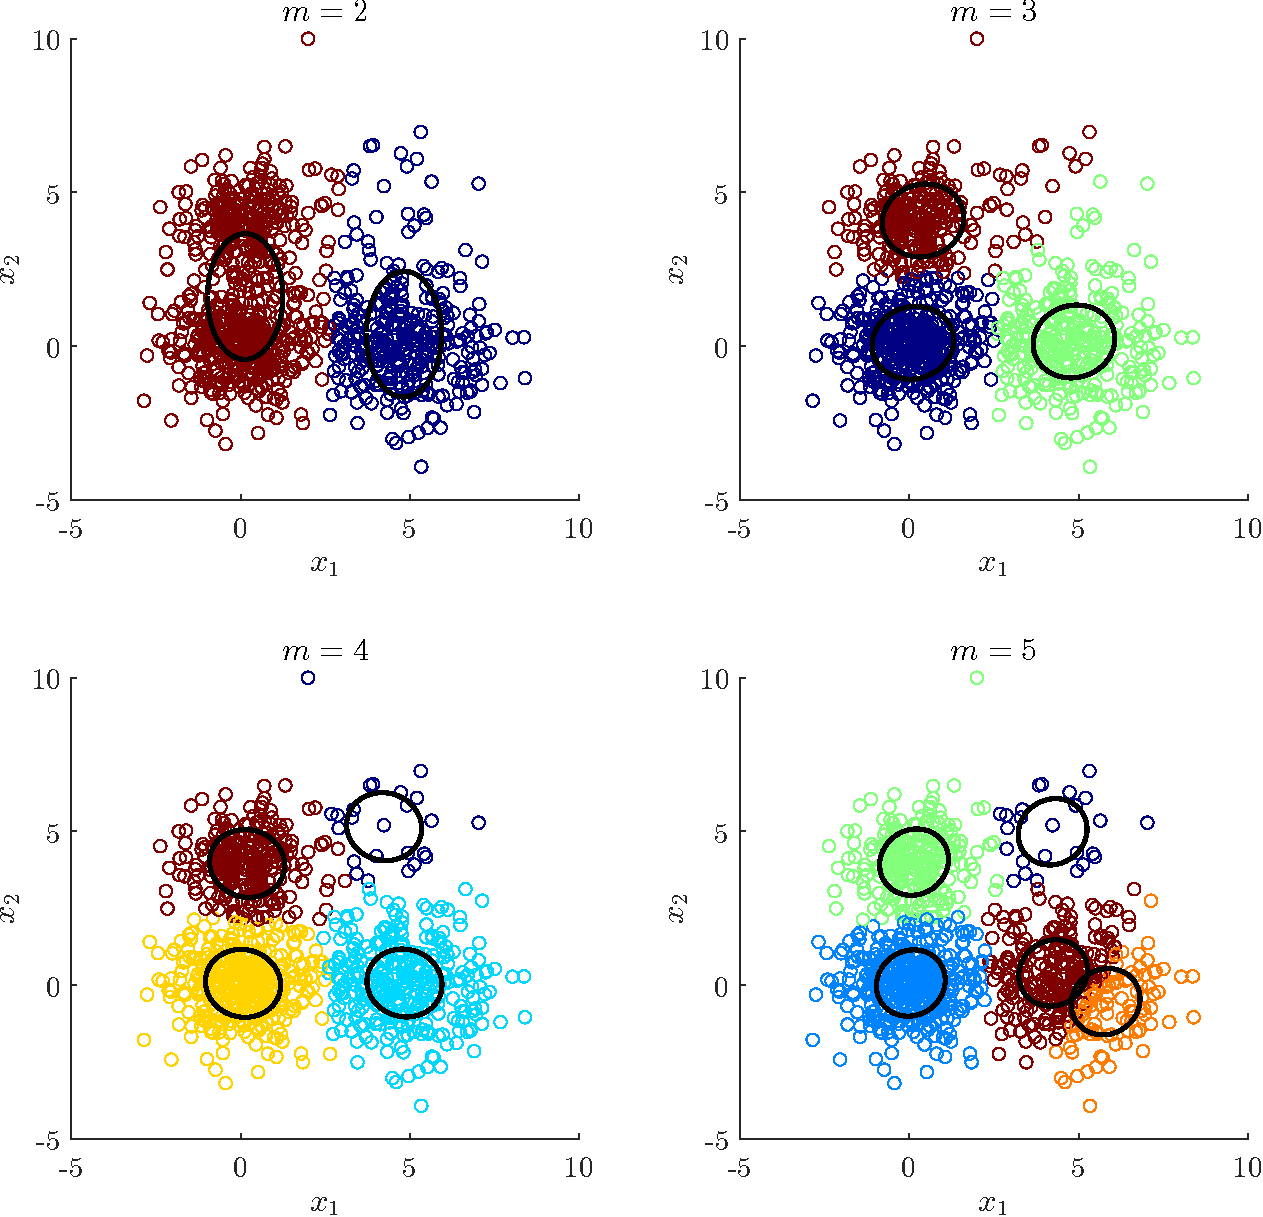
\includegraphics[width=6in]{gmmem-eqcov.pdf}
  \caption{使用修改的 EM 算法对 GMM 模型进行估计}
  \label{fig:gmmemeq}
\end{figure}

BIC 计算结果如表 \ref{tab:biceq} 所示, 可知当 $m=4$ 时, BIC 最小, 即 $m=4$ 仍为最恰当的模型参数. 

\begin{table}[htbp]
  \centering
  \caption{不同参数 $m$ 取值对应的 BIC 数值}
  \label{tab:biceq}
  \begin{tabular}{ccccc}
    \hline
        & $m=2$ & $m=3$ & $m=4$ & $m=5$ \\
    \hline
    BIC & 8597.40 & 8463.17 & 8397.21 & 8415.93\\
    \hline
  \end{tabular}
\end{table}

\newpage
\section*{Programming 2 (Missing Data)}

4. Suppose we know that the ten data points in category $\omega_1$ in Tab.~\ref{tab:sampledata} come from a three-dimensional Gaussian. Suppose, however, that we do not have access to the $x_3$ components for the even-numbered data points.

\begin{table}[h]
  \centering
  \caption{样本数据点}
  \label{tab:sampledata}
  \begin{tabular}{c|ccc}
		\hline
		&  &  $\omega_1$ & \\
		point & $x_1$ & $x_2$ & $x_3$ \\
		\hline
		1 & 0.42 & -0.087 & 0.58\\
		2 & -0.2 & -3.3 & -3.4\\
		3 & 1.3 & -0.32 & 1.7\\
		4 & 0.39 & 0.71 & 0.23\\
		5 & -1.6 & -5.3 & -0.15\\
		6 & -0.029 & 0.89 & -4.7\\
		7 & -0.23 & 1.9 & 2.2\\
		8 & 0.27 & -0.3 & -0.87\\
		9 & -1.9 & 0.76 & -2.1\\
		10 & 0.87 & -1.0 & -2.6 \\
		\hline
	\end{tabular}
\end{table}

4.1. Write an EM program to estimate the mean and covariance of the distribution. Start your estimate with $\bm{\mu}^0=\bm{0}$ and $\bm{\Sigma}^0=\bm{I}$, the three-dimensional identity matrix.

解: 记 $O=\{1,3,5,7,9\}$, $E=\{2,4,6,8,10\}$. 偶数点的 $x_3$ 数据丢失, 则令 $x_{i3}$, $i\in E$ 为隐变量, 并令 $q(\cdot)$ 表示其概率分布, 则对数似然函数为
\begin{equation}
  \begin{aligned}
    H(\theta)
    &=\sum_{i\in O}\ln p(x_{i1},x_{i2},x_{i3}|\theta)+\sum_{i\in E}\ln p(x_{i1},x_{i2}|\theta)\\
    &=\sum_{i\in O}\ln p(x_{i1},x_{i2},x_{i3}|\theta)+\sum_{i\in E}\ln\int_{-\infty}^\infty p(x_{i1},x_{i2},x_{i3}|\theta)\mathrm{d}x_{i3}\\
    &=\sum_{i\in O}\ln p(x_{i1},x_{i2},x_{i3}|\theta)+\sum_{i\in E}\ln\int_{-\infty}^\infty q(x_{i3})\frac{p(x_{i1},x_{i2},x_{i3}|\theta)}{q(x_{i3})}\mathrm{d}x_{i3}\\
    &\gs\sum_{i\in O}\ln p(x_{i1},x_{i2},x_{i3}|\theta)+\sum_{i\in E}\int_{-\infty}^\infty q(x_{i3})\ln\frac{p(x_{i1},x_{i2},x_{i3}|\theta)}{q(x_{i3})}\mathrm{d}x_{i3}\\
  \end{aligned}
\end{equation}

由此可得 $Q$ 函数为
\begin{equation}
  Q(\theta^{(k)},\theta)=\sum_{i\in O}\ln p(x_{i1},x_{i2},x_{i3}|\theta)+\sum_{i\in E}\int_{-\infty}^\infty p(x_{i3}|x_{i1},x_{i2},\theta^{(k)})\ln p(x_{i1},x_{i2},x_{i3}|\theta)\mathrm{d}x_{i3}
\end{equation}

令 $x_i=(x_{i1},x_{i2},x_{i3})^{\top}$, $\mu=(\mu_1,\mu_2,\mu_3)^{\top}$, 则
\begin{equation}
  \ln p(x_{i1},x_{i2},x_{i3}|\theta)=\ln p(x_i|\theta)=-\frac{3}{2}\ln(2\pi)+\frac{1}{2}\ln|\Sigma^{-1}|-\frac{1}{2}(x_i-\mu)^{\top}\Sigma^{-1}(x_i-\mu)
\end{equation}

$Q$ 对 $\mu$ 的偏导数为
\begin{equation}
  \begin{aligned}
    \frac{\partial Q(\theta^{(k)},\theta)}{\partial \mu}
    &=\sum_{i\in O}\Sigma^{-1}(x_i-\mu)+\sum_{i\in E}\int_{-\infty}^\infty p(x_{i3}|x_{i1},x_{i2},\theta^{(k)})\Sigma^{-1}(x_i-\mu)\mathrm{d}x_{i3}\\
    &=\sum_{i\in O}\Sigma^{-1}
      \begin{pmatrix}
        x_{i1}-\mu_1\\
        x_{i2}-\mu_2\\
        x_{i3}-\mu_3\\
      \end{pmatrix}
    +\sum_{i\in E}\Sigma^{-1}
      \begin{pmatrix}
        x_{i1}-\mu_1\\
        x_{i2}-\mu_2\\
        \displaystyle\int_{-\infty}^\infty x_{i3} p(x_{i3}|x_{i1},x_{i2},\theta^{(k)})\mathrm{d}x_{i3}-\mu_3\\
      \end{pmatrix}\\
    &=\Sigma^{-1}
      \begin{pmatrix}
        \displaystyle\sum_{i=1}^{10}(x_{i1}-\mu_1)\\
        \displaystyle\sum_{i=1}^{10}(x_{i2}-\mu_2)\\
        \displaystyle\sum_{i\in O}x_{i3}+\sum_{i\in E}\mathbb{E}(x_{i3}|x_{i1},x_{i2},\theta^{(k)})-\sum_{i=1}^{10}\mu_3\\
      \end{pmatrix}
  \end{aligned}
\end{equation}

令此偏导数为 0, 有
\begin{equation}
  \begin{aligned}
    \mu_1&=\frac{1}{10}\sum_{i=1}^{10}x_{i1}\\
    \mu_2&=\frac{1}{10}\sum_{i=1}^{10}x_{i2}\\
    \mu_3&=\frac{1}{10}\sum_{i\in O}x_{i3}+\frac{1}{10}\sum_{i\in E}\mathbb{E}(x_{i3}|x_{i1},x_{i2},\theta^{(k)})\\
  \end{aligned}
\end{equation}

由高斯分布的性质可知, 高斯分布的条件分布仍为高斯分布, 记
\begin{equation}
  \Sigma^{(k)}=
  \begin{bmatrix}
    \Sigma_{12,12}^{(k)} & \Sigma_{12,3}^{(k)}\\
    \Sigma_{3,12}^{(k)}  & \Sigma_{3,3}^{(k)} \\
  \end{bmatrix}
\end{equation}

则由相关公式 \cite{b1,b2,b3} 可知
\begin{equation}
  \mathbb{E}(x_{i3}|x_{i1},x_{i2},\theta^{(k)})=\mu_3^{(k)}+\Sigma_{3,12}^{(k)}\left[\Sigma_{12,12}^{(k)}\right]^{-1}
  \begin{pmatrix}
    x_{i1}-\mu_1^{(k)}\\
    x_{i2}-\mu_2^{(k)}\\
  \end{pmatrix}
\end{equation}

所以
\begin{equation}
  \mu_3=\frac{1}{10}\sum_{i\in O}x_{i3}+\frac{1}{10}\sum_{i\in E}\left[\mu_3^{(k)}+\Sigma_{3,12}^{(k)}\left[\Sigma_{12,12}^{(k)}\right]^{-1}
  \begin{pmatrix}
    x_{i1}-\mu_1^{(k)}\\
    x_{i2}-\mu_2^{(k)}\\
  \end{pmatrix}\right]
\end{equation}

令
\begin{equation}
  N_i^{(k)}=(x_i-\mu^{(k+1)})(x_i-\mu^{(k+1)})^{\top},\quad M_i=\Sigma-N_i^{(k)}
\end{equation}

则 $Q$ 对 $\Sigma^{-1}$ 的偏导数为
\begin{equation}
  \begin{aligned}
    \frac{\partial Q(\theta^{(k)},\theta)}{\partial\Sigma^{-1}}
    &=\sum_{i\in O}\frac{1}{2}\big[2M_i-\diag(M_i)\big]+\sum_{i\in E}\int_{-\infty}^\infty p(x_{i3}|x_{i1},x_{i2},\theta^{(k)})\frac{1}{2}\big[2M_i-\diag(M_i)\big]\mathrm{d}x_{i3}
  \end{aligned}
\end{equation}

令此偏导数为 0, 有
\begin{equation}
  \sum_{i\in O}M_i+\sum_{i\in E}\int_{-\infty}^\infty p(x_{i3}|x_{i1},x_{i2},\theta^{(k)})M_i\mathrm{d}x_{i3}=0
\end{equation}

即
\begin{equation}
  \sum_{i\in O}(\Sigma-N_i^{(k)})+\sum_{i\in E}\int_{-\infty}^\infty p(x_{i3}|x_{i1},x_{i2},\theta^{(k)})(\Sigma-N_i^{(k)})\mathrm{d}x_{i3}=0
\end{equation}

由概率密度函数积分为 1, 可得
\begin{equation}
  \sum_{i=1}^{10}\Sigma-\sum_{i\in O}N_i^{(k)}-\sum_{i\in E}\int_{-\infty}^\infty p(x_{i3}|x_{i1},x_{i2},\theta^{(k)})N_i^{(k)}\mathrm{d}x_{i3}=0
\end{equation}

所以
\begin{equation}
  \begin{aligned}
    \Sigma
    &=\frac{1}{10}\sum_{i\in O}N_i^{(k)}+\frac{1}{10}\sum_{i\in E}\int_{-\infty}^\infty p(x_{i3}|x_{i1},x_{i2},\theta^{(k)})N_i^{(k)}\mathrm{d}x_{i3}\\
    &\triangleq\frac{1}{10}\sum_{i\in O}N_i^{(k)}+\frac{1}{10}\sum_{i\in E}W_i^{(k)}\\
  \end{aligned}
\end{equation}

其中
\begin{equation}
  \begin{aligned}
    W_i^{(k)}
    &=\int_{-\infty}^\infty p(x_{i3}|x_{i1},x_{i2},\theta^{(k)})(x_i-\mu^{(k+1)})(x_i-\mu^{(k+1)})^{\top}\mathrm{d}x_{i3}\\
    &=\int_{-\infty}^\infty p(x_{i3}|x_{i1},x_{i2},\theta^{(k)})
      \begin{bmatrix}
        (x_{i1}-\mu_1)^2 & (x_{i1}-\mu_1)(x_{i2}-\mu_2) & (x_{i1}-\mu_1)(x_{i3}-\mu_3)\\
        (x_{i2}-\mu_2)(x_{i1}-\mu_1) & (x_{i2}-\mu_2)^2 & (x_{i2}-\mu_2)(x_{i3}-\mu_3)\\
        (x_{i3}-\mu_3)(x_{i1}-\mu_1) & (x_{i3}-\mu_3)(x_{i2}-\mu_2) & (x_{i3}-\mu_3)^2\\
      \end{bmatrix}
    \mathrm{d}x_{i3}\\
  \end{aligned}
\end{equation}

记
\begin{equation}
  E_i^{(k)}\triangleq\mathbb{E}(x_{i3}|x_{i1},x_{i2},\theta^{(k)})=\mu_3^{(k)}+\Sigma_{3,12}^{(k)}\left[\Sigma_{12,12}^{(k)}\right]^{-1}
    \begin{pmatrix}
      x_{i1}-\mu_1^{(k)}\\
      x_{i2}-\mu_2^{(k)}\\
    \end{pmatrix}
\end{equation}

以及
\begin{equation}
  D_i^{(k)}\triangleq\mathrm{Var}(x_{i3}|x_{i1},x_{i2},\theta^{(k)})=\Sigma_{3,3}^{(k)}-\Sigma_{3,12}^{(k)}\left[\Sigma_{12,12}^{(k)}\right]^{-1}\Sigma_{12,3}^{(k)}
\end{equation}

则由期望和方差的定义得到
\begin{equation}
  \begin{aligned}
    W_i^{(k)}
    &=
    \begin{bmatrix}
      (x_{i1}-\mu_1)^2 & (x_{i1}-\mu_1)(x_{i2}-\mu_2) & (x_{i1}-\mu_1)\left(E_i^{(k)}-\mu_3\right)\\[2mm]
      (x_{i2}-\mu_2)(x_{i1}-\mu_1) & (x_{i2}-\mu_2)^2 & (x_{i2}-\mu_2)\left(E_i^{(k)}-\mu_3\right)\\
      \left(E_i^{(k)}-\mu_3\right)(x_{i1}-\mu_1) & \left(E_i^{(k)}-\mu_3\right)(x_{i2}-\mu_2) & D_i^{(k)}+\left(E_i^{(k)}\right)^2-2\mu_3E_i^{(k)}+\mu_3^2\\
    \end{bmatrix}
  \end{aligned}
\end{equation}

综上所述, 有
\begin{equation}
  \begin{aligned}
    \mu_1^{k+1}&=\frac{1}{10}\sum_{i=1}^{10}x_{i1}\\
    \mu_2^{k+1}&=\frac{1}{10}\sum_{i=1}^{10}x_{i2}\\
    \mu_3^{k+1}&=\frac{1}{10}\sum_{i\in O}x_{i3}+\frac{1}{10}\sum_{i\in E}E_i^{(k)}\\
    \Sigma^{k+1}&=\frac{1}{10}\sum_{i\in O}N_i^{(k)}+\frac{1}{10}\sum_{i\in E}W_i^{(k)}\\
  \end{aligned}
\end{equation}

编写程序, 得到估计的均值向量和协方差矩阵分别为
\begin{equation}
  \hat{\mu}=
  \begin{pmatrix}
    -0.0709\\
    -0.6047\\
    0.7728\\
  \end{pmatrix},
  \quad
  \hat{\Sigma}=
  \begin{bmatrix}
    0.9062 & 0.5678 & 0.8814 \\
    0.5678 & 4.2007 & 0.4621 \\
    0.8814 & 0.4621 & 1.7828 \\
  \end{bmatrix}
\end{equation}

4.2. Compare your final estimation with the case when we remove all even-numbered data points (2, 4, 6, 8, 10).

解: 均值向量和协方差矩阵分别为
\begin{equation}
  \hat{\mu}=
  \begin{pmatrix}
    -0.4020\\
    -0.6094\\
    0.4460\\
  \end{pmatrix},
  \quad
  \hat{\Sigma}=
  \begin{bmatrix}
    1.4563 & 0.9843 & 1.4148 \\
    0.9843 & 6.1061 & 0.8287 \\
    1.4148 & 0.8287 & 2.3009 \\
  \end{bmatrix}
\end{equation}

全部偶数数据点的缺失导致均值和协方差矩阵的估计有了很大的变化, 除了 $x_2$ 的均值估计基本保持不变外, 其余数值均发生了较大的变化, 与只缺失 $x_3$ 的偶数数据点相比近乎是两个不同的模型了, 可以看出数据点的个数对模型参数的估计有较大的影响.

4.3. Compare your final estimation with the case when there are no missing data, namely we have access to all $x_3$.

解: 均值向量和协方差矩阵分别为
\begin{equation}
  \hat{\mu}=
  \begin{pmatrix}
    -0.0709\\
    -0.6047\\
    -0.9110\\
  \end{pmatrix},
  \quad
  \hat{\Sigma}=
  \begin{bmatrix}
    0.9062 & 0.5678 & 0.3941 \\
    0.5678 & 4.2007 & 0.7337 \\
    0.3941 & 0.7337 & 4.5419 \\
  \end{bmatrix}
\end{equation}

由于只缺失第三维的部分数据, 所以前两维的均值和协方差估计都是准确的, 而第三维有明显的误差, 且误差较大. 这主要是因为缺失的五个数据, 恰好都是 $x_3$ 比较小的数据, 导致估计有了较大的误差.

% Reference
\begin{thebibliography}{1}
  \bibitem{b1}{Flying pig. Deriving the conditional distributions of a multivariate normal distribution, 2012. \href{https://stats.stackexchange.com/questions/30588}{https://stats.stackexchange.com/questions/30588}}
  \bibitem{b2}{Ruye Wang. Marginal and conditional distributions of multivariate normal distribution, 2006. \href{http://fourier.eng.hmc.edu/e161/lectures/gaussianprocess/node7.html}{http://fourier.eng.hmc.edu/e161/lectures/gaussianprocess/node7.html}}
  \bibitem{b3}{Steffen Lauritzen. The Multivariate Gaussian Distribution, 2009. \href{http://www.stats.ox.ac.uk/~steffen/teaching/bs2HT9/gauss.pdf}{http://www.stats.ox.ac.uk/~steffen/teaching/bs2HT9/gauss.pdf}}
\end{thebibliography}

\end{document}
